\documentclass[border=0.125cm]{standalone}
\usepackage{tikz}
\usetikzlibrary{positioning}
\begin{document}

\tikzset{%
  every neuron/.style={
    circle,
    draw,
    minimum size=1cm
  },
  neuron missing/.style={
    draw=none, 
    scale=4,
    text height=0.333cm,
    execute at begin node=\color{black}$\vdots$
  },
}

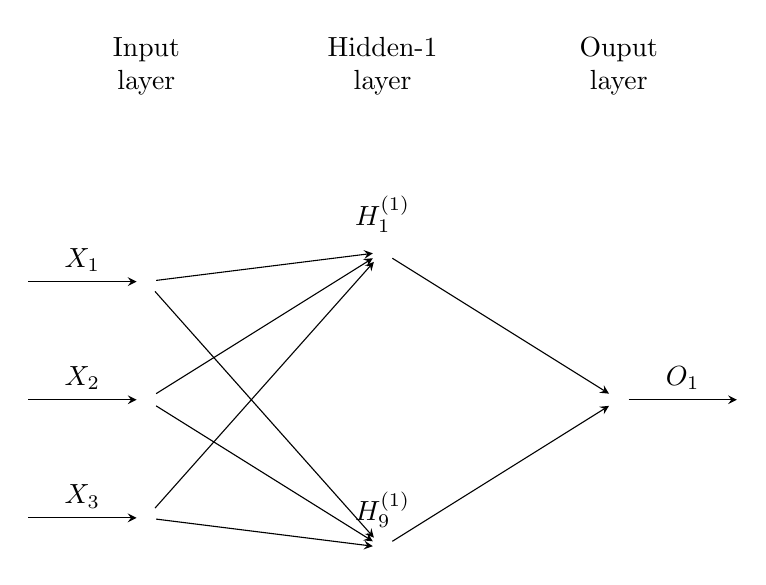
\begin{tikzpicture}[x=1.5cm, y=1.5cm, >=stealth]

% input layer
\foreach \m/\l [count=\y] in {1,2,3}
  \node [every neuron/.try, neuron \m/.try] (input-\m) at (0,1.5-\y) {};

% hidden layer 1
\foreach \m [count=\y] in {1,missing,2}
  \node [every neuron/.try, neuron \m/.try ] (hidden-\m) at (2,2-\y*1.25) {};


% output layer
\foreach \m [count=\y] in {1}
  \node [every neuron/.try, neuron \m/.try ] (output-\m) at (4,0.5-\y) {};

% input layer labeling
\foreach \l [count=\i] in {1,2,3}
  \draw [<-] (input-\i) -- ++(-1,0)
    node [above, midway] {$X_\l$};

% hidden layer 1 labeling
\foreach \l [count=\i] in {1,9}
  \node [above] at (hidden-\i.north) {$H^{(1)}_\l$};


% output layer labeling
\foreach \l [count=\i] in {1}
  \draw [->] (output-\i) -- ++(1,0)
    node [above, midway] {$O_\l$};

% arrows from input to hidden layer 1
\foreach \i in {1,2,3}
  \foreach \j in {1,...,2}
    \draw [->] (input-\i) -- (hidden-\j);



% arrows from hidden layer 2 to output layer
\foreach \i in {1,...,2}
  \foreach \j in {1}
    \draw [->] (hidden-\i) -- (output-\j);



\foreach \l [count=\x from 0] in {Input, Hidden-1, Ouput}
  \node [align=center, above] at (\x*2,2) {\l \\ layer};

\end{tikzpicture}

\end{document}